\begin{figure}[H]
\centering
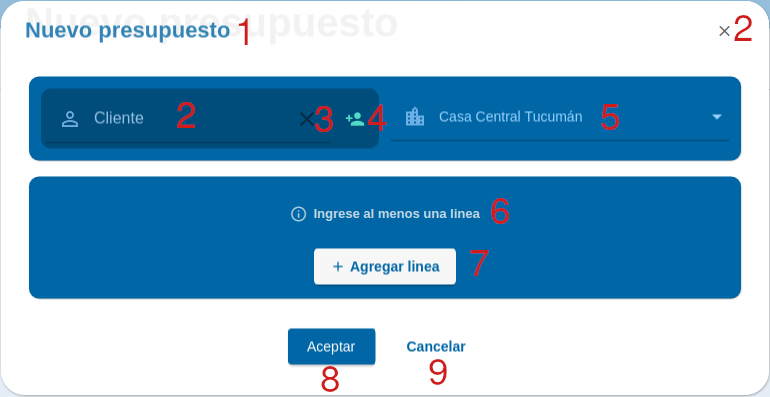
\includegraphics[width=\textwidth,height=\textheight,keepaspectratio]{Escenarios/AD-04-00}
\caption{Escenario - AD-04-00}
\label{fig:AD-04-00}
\end{figure}
Este es el escenario que permite a los usuarios crear y modificar presupuestos, el campo \textbf{AD-04-01} indicará la acción que se va a realizar, pudiendo ser 'Nuevo presupuesto' o 'Editar presupuesto'. Con el botón \textbf{AD-04-02} se podrá cerrar la ventana y volver al escenario \textbf{AD-03-00}.
El campo \textbf{AD-04-03} permite al usuario indicar el cliente para el cúal se esta creando el presupuesto o indicar el nuevo cliente en caso que se esté editando el presupuesto. El botón \textbf{AD-04-04} permite crear un nuevo cliente navegando al escenario \textbf{AD-29-00}. La lista desplegable \textbf{AD-04-05} permite al usuario indicar la ubicación en la cúal se esta creando el presupuesto o bien modificar la misma. El campo \textbf{AD-04-06} se muestra cuando el presupuesto no tiene asociado ninguna linea de presupuesto. El boton \textbf{AD-04.07} permite al usuario crear una linea de venta y asociarla al presupuesto, navega al escenario \textbf{AD-05-00}. Si el usuario hace click en el botón \textbf{AD-04-08} creará el presupuesto y navegará al escenario \textbf{AD-07-00}, si hace click en el botón \textbf{AD-04-09} cerrará la ventana navegando al escenario \textbf{AD-03-00}.
\clearpage
